\documentclass[12pt]{article}\usepackage[]{graphicx}\usepackage[]{color}
% maxwidth is the original width if it is less than linewidth
% otherwise use linewidth (to make sure the graphics do not exceed the margin)
\makeatletter
\def\maxwidth{ %
  \ifdim\Gin@nat@width>\linewidth
    \linewidth
  \else
    \Gin@nat@width
  \fi
}
\makeatother

\definecolor{fgcolor}{rgb}{0.345, 0.345, 0.345}
\newcommand{\hlnum}[1]{\textcolor[rgb]{0.686,0.059,0.569}{#1}}%
\newcommand{\hlstr}[1]{\textcolor[rgb]{0.192,0.494,0.8}{#1}}%
\newcommand{\hlcom}[1]{\textcolor[rgb]{0.678,0.584,0.686}{\textit{#1}}}%
\newcommand{\hlopt}[1]{\textcolor[rgb]{0,0,0}{#1}}%
\newcommand{\hlstd}[1]{\textcolor[rgb]{0.345,0.345,0.345}{#1}}%
\newcommand{\hlkwa}[1]{\textcolor[rgb]{0.161,0.373,0.58}{\textbf{#1}}}%
\newcommand{\hlkwb}[1]{\textcolor[rgb]{0.69,0.353,0.396}{#1}}%
\newcommand{\hlkwc}[1]{\textcolor[rgb]{0.333,0.667,0.333}{#1}}%
\newcommand{\hlkwd}[1]{\textcolor[rgb]{0.737,0.353,0.396}{\textbf{#1}}}%
\let\hlipl\hlkwb

\usepackage{framed}
\makeatletter
\newenvironment{kframe}{%
 \def\at@end@of@kframe{}%
 \ifinner\ifhmode%
  \def\at@end@of@kframe{\end{minipage}}%
  \begin{minipage}{\columnwidth}%
 \fi\fi%
 \def\FrameCommand##1{\hskip\@totalleftmargin \hskip-\fboxsep
 \colorbox{shadecolor}{##1}\hskip-\fboxsep
     % There is no \\@totalrightmargin, so:
     \hskip-\linewidth \hskip-\@totalleftmargin \hskip\columnwidth}%
 \MakeFramed {\advance\hsize-\width
   \@totalleftmargin\z@ \linewidth\hsize
   \@setminipage}}%
 {\par\unskip\endMakeFramed%
 \at@end@of@kframe}
\makeatother

\definecolor{shadecolor}{rgb}{.97, .97, .97}
\definecolor{messagecolor}{rgb}{0, 0, 0}
\definecolor{warningcolor}{rgb}{1, 0, 1}
\definecolor{errorcolor}{rgb}{1, 0, 0}
\newenvironment{knitrout}{}{} % an empty environment to be redefined in TeX

\usepackage{alltt}

%%% draft settings

% line numbers
\usepackage{lineno}
\linenumbers

% double spacing
\usepackage{setspace}
\doublespacing

% figures
\usepackage{graphicx}
\usepackage{amsmath,amssymb}

%%% code
\newcommand{\code}[1]{\texttt{{#1}}}
% package
\newcommand{\package}[1]{\texttt{{#1::}}}
% function
\newcommand{\function}[1]{\texttt{{::#1}}}
% package::function
\newcommand{\packagefn}[2]{\texttt{{#1::#2}}}

% title
\title{A computational way station for reporting network meta-analyses}
\author{Charles T. Gray, Gavin Stewart, Matthew Grainger}
\IfFileExists{upquote.sty}{\usepackage{upquote}}{}
\begin{document}







\maketitle


\section{Network meta-analysis reporting}\label{sec:nma}

% why is it important

Pairwise analyses between treatment and control, exposed and unexposed, intervention and no intervention, are conventionally undertaken with meta-analysis in fields such as ecology, medicine, and the social sciences~\cite{borenstein_introduction_2011}. Network meta-analysis provides a means of comparing three or more treatments or interventions, including control or placebo~\cite{higgins2019cochrane}. The question answered by a network meta-analysis is not \emph{if} a treatment works, but \emph{which} treatments perform better, comparatively~\cite{harrer_doing_2019}. A particularly useful aspect of network meta-analysis is combining the results of more than one pairwise analysis and constructing indirect comparisons, where pairwise evidence is unavailable, from a network of direct comparisons. An example of direct comparisons provided by existing evidence is shown in Figure \ref{fig:network}. Network meta-analysis converts the network to a complete graph, where all treatments are compared with all other treatments, that is, every node connects to every other node via direct or indirect comparison.

\begin{figure}
\centering
\begin{knitrout}
\definecolor{shadecolor}{rgb}{0.969, 0.969, 0.969}\color{fgcolor}
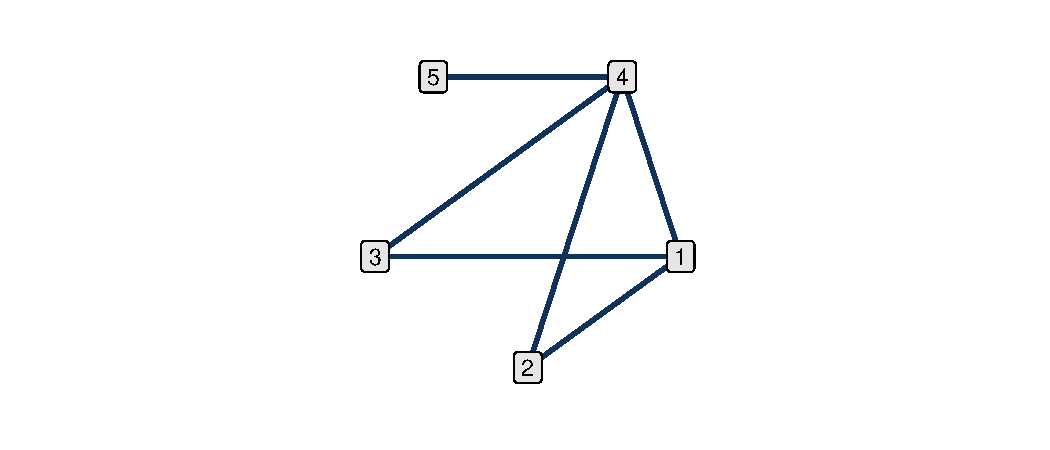
\includegraphics[width=\maxwidth]{figure/network-1} 

\end{knitrout}
\caption{This network shows the direct evidence provided by pairwise comparisons in seven studies on treatments for Parkinson's disease~\cite{phillippo_multinma_2020}. Each node represents a treatment, including one placebo, represented by the fourth node. Where there is an edge connecting two treatment nodes, there exists a pairwise comparison in the literature between these two treatments. Where there is no edge connecting the nodes of the network, there is no direct evidence.}
\label{fig:network}
\end{figure}

Software to implement network meta-analyses are relatively new and do not provide complete toolchains for specific protocols, such as reporting results according to Cochrane's handbook~\cite{higgins2019cochrane}. For example, the handbook recommends reporting the network of direct evidence, for which the R package \package{multinma} includes a tool~\cite{phillippo_multinma_2020}, an example of which is shown in Figure \ref{fig:network}. However, the handbook also recommends reporting a \textbf{contribution matrix} of the percentage of each study's contribution to the estimated overall effect, and this is not provided as a visualisation tool with \package{multinma}.

Furthermore, open source scientific software is shifting from all-purpose packages for an entire analysis, such as \package{metafor}, to smaller task-specific software packages. One method of aggregation of tools is a \textbf{metapackage}, such as \package{tidyverse}~\cite{wickham_tidyverse_2017}, for data engineering, which comprises a number of packages that each pertain to different problems, such as \package{ggplot2} for data visualisation, and \package{dplyr} for Boolean data manipulation. Here we explore another way of aggregating resources, for the specific purpose of network meta-analysis reporting: a computational \textbf{way station}, a temporary resting place between two points of travel, of toolchains and tool development. Since protocols and tools are are still being developed, this is a way station between a single person's analysis, and a resource that is definitive for all practitioners to follow.

\subsection{A snapshot of a living resource}

In this manuscript, we next describe the gaps in the toolchain for implementing network meta-analysis via R according to Cochrane's reporting standards. Standards for network meta-analysis are not, however, fixed, but in development, and Cochrane's reporting standards may not be appropriate for, say, ecological network meta-analyses. Thus, instead of aiming to provide a complete toolchain for network meta-analysis, we instead propose a computational way station as a meeting place for stakeholders with different priorities to provide perspective and collaborate. This way station is a \textbf{living resource}, in anticipation of future updates following stakeholder input and computational development, comprising multiple points of access:

\begin{description}
\item[website] A website with vignettes of toolchains. Currently the existing solutions for Cochrane's reporting standards are provided, however there is scope for future vignettes for network meta-analyses according to other discipline or organisational protocols.
\item[open source code repository] Source code is provided for toolchains and software extensions.
\item[contributing] Detailed instructions for different stakeholders with varying levels of mathematical and computational training to contribute.
\item[issues] In addition to the source code, the issues associated with the code repository provide a public record for discussions.
\end{description}

Living resources provide a solution to the problem of overabundance of systematic reviews, flooding literature to the point that decision makers are unsure of where to look~\cite{gopalakrishnan_systematic_2013, moher_problem_2013, moller_are_2018, richards_too_2018}. Consider Covid-19, where in the first 88 days after naming the disease, there already existed 88 systematic reviews, one for every day since the disease was named~\cite{naumann_too_2021}. Cochrane's COVID-NMA initiative (https://covid-nma.com/) is a living synthesis solution to this problem, via network meta-analysis of regularly updated Covid-19 research~\cite{boutron_covid-nma_2020}.

\package{nmareporting} is also a living resource, but to solve a different problem. How to bring people together for open scientific collaboration when not all the solutions exist. As a package it is not ready for CRAN, and may never be intended for CRAN. In some ways similar to the \package{rethinking} package the accompanies the canonical\footnote{
At the time of writing \emph{Statistical Rethinking} has 1243 citations.
} text, \emph{Statistical Rethinking}, the intention of this software is not to ship a polished piece of software to CRAN, or a publish a manuscript with a definitive toolchain~\cite{statrethinkingbook}. Rather, this manuscript provides a snapshot of a living resource for open collaboration on network meta-analysis reporting.

\section{Toolchain gaps in Cochrane reporting standards}

There exist several software packages for conduction network meta-analysis in R; for example, \package{gemtc}~\cite{valkenhoef_gemtc_2020}, \package{multinma}~\cite{phillippo_multinma_2020}, and \package{netmeta}~\cite{rucker_netmeta_2021}. Different tools will no doubt have unique advantages and disadvantages, however, there is no one tool for all reporting standards for a Cochrane network meta-analysis. Furthermore, visualisations and reporting for meta-analysis are still being developed.

\subsection{Missing tables and improved visualisations}

% orchard plots, caterpillar plots

Cochrane recommends reporting the percentage each study contributes to the overall estimated effect via a \textbf{contribution matrix}, shown in Figure \ref{fig:cmatrix}.

\begin{figure}
\centering
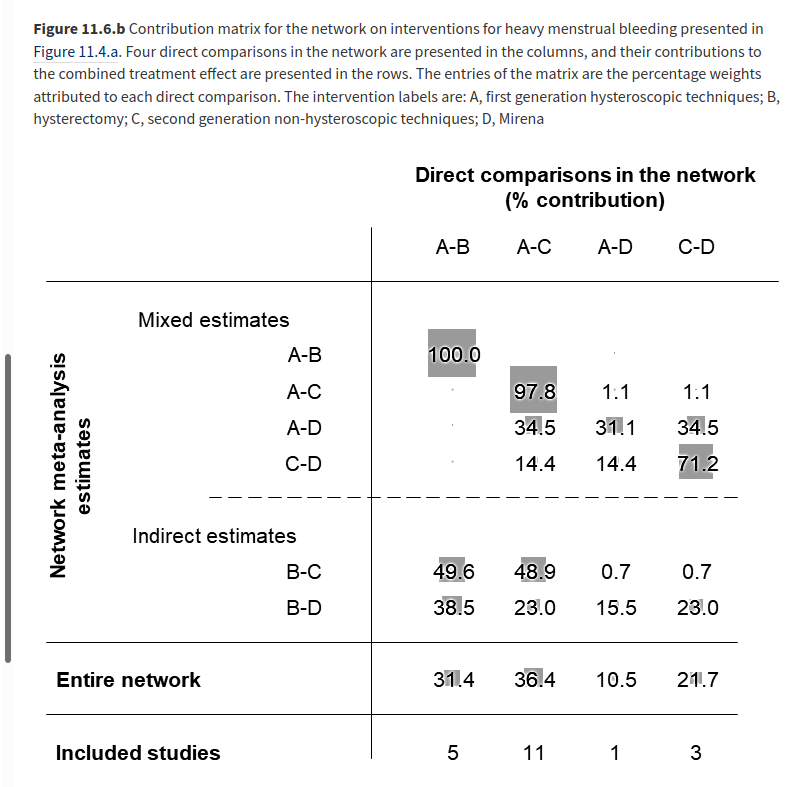
\includegraphics[width=0.5\textwidth]{contribution-matrix}
\caption{A contribution matrix shows what percentage each study contributes to the overall estimated effect in a network meta-analysis. This is the example given in the Cochrane Handbook~\cite{higgins2019cochrane}.}
\label{fig:cmatrix}
\end{figure}

The \package{netmeta} package has tools for contribution matrices, but if one is performing the analysis with, say, \package{multinma}, it is unclear how to piece together the tools to produce a complete set of Cochrane reporting.

\emph{Gav, is the contribution matrix only for frequentist analysis?}

Visualisations, too, are still in development. A recent improvement on standard forest plots are orchard plots which contain not only credible intervals, but prediction intervals, and group studies categorically, particularly useful for large meta-analyses~\cite{nakagawa_orchard_2021}. \package{nmareporting} is a place where implementation of orchard plots for network meta-analysis can be developed.

\subsection{Sensitivity}





Sensitivity in network meta-analysis measures how much the studies agree in results. A standard approach to measuring this is a `leave one out analysis'~\cite{borenstein_introduction_2011}, shown in Figure \ref{fig:one}, where a study is randomly selected to be omitted, and the meta-analysis is rerun to see if the results differ. We randomly\footnote{
This manuscript is fully reproducible, with all analyses and code embedded in the document. The source for this manuscript can be found here: https://github.com/softloud/nmareporting/blob/master/manuscript/draft/nmarep-ms.Rnw.
} select

\begin{knitrout}
\definecolor{shadecolor}{rgb}{0.969, 0.969, 0.969}\color{fgcolor}\begin{kframe}
\begin{verbatim}
## [1] "study_1"
\end{verbatim}
\end{kframe}
\end{knitrout}

to remove from the analysis.

\begin{figure}
\begin{knitrout}
\definecolor{shadecolor}{rgb}{0.969, 0.969, 0.969}\color{fgcolor}
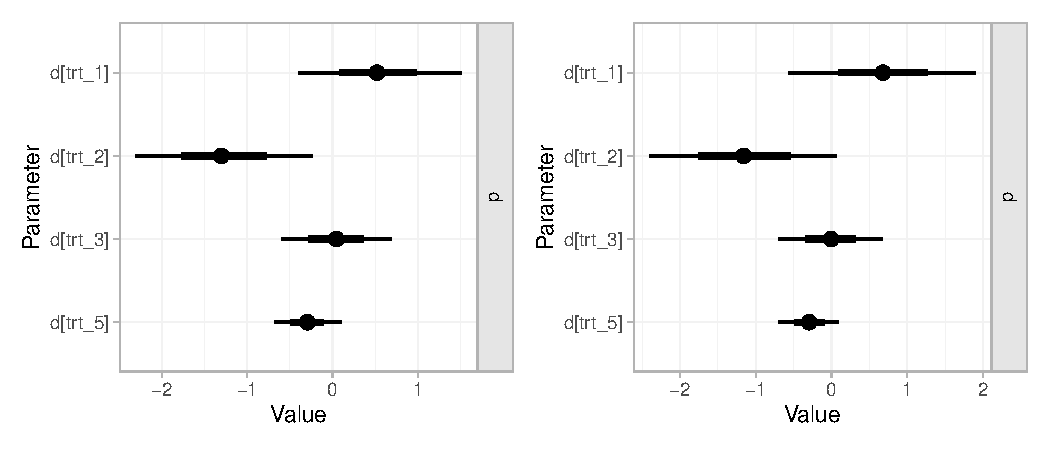
\includegraphics[width=\maxwidth]{figure/forest-1} 

\end{knitrout}

\caption{On the left is a forest plot of all analyses. On the right is a forest plot of the analysis with a randomly selected study omitted.}
\label{fig:one}
\end{figure}

In this case, there is little disagreement between the studies. However, it does raise the question of what the analysis would report if another study were omitted, and, indeed, what if more than one study were omitted? In Figure \ref{fig:leavem}, we provide aggregation of rankings of network meta-analyses run on all subsets, of size three or greater, of the studies.











\begin{figure}
\centering
\begin{knitrout}
\definecolor{shadecolor}{rgb}{0.969, 0.969, 0.969}\color{fgcolor}
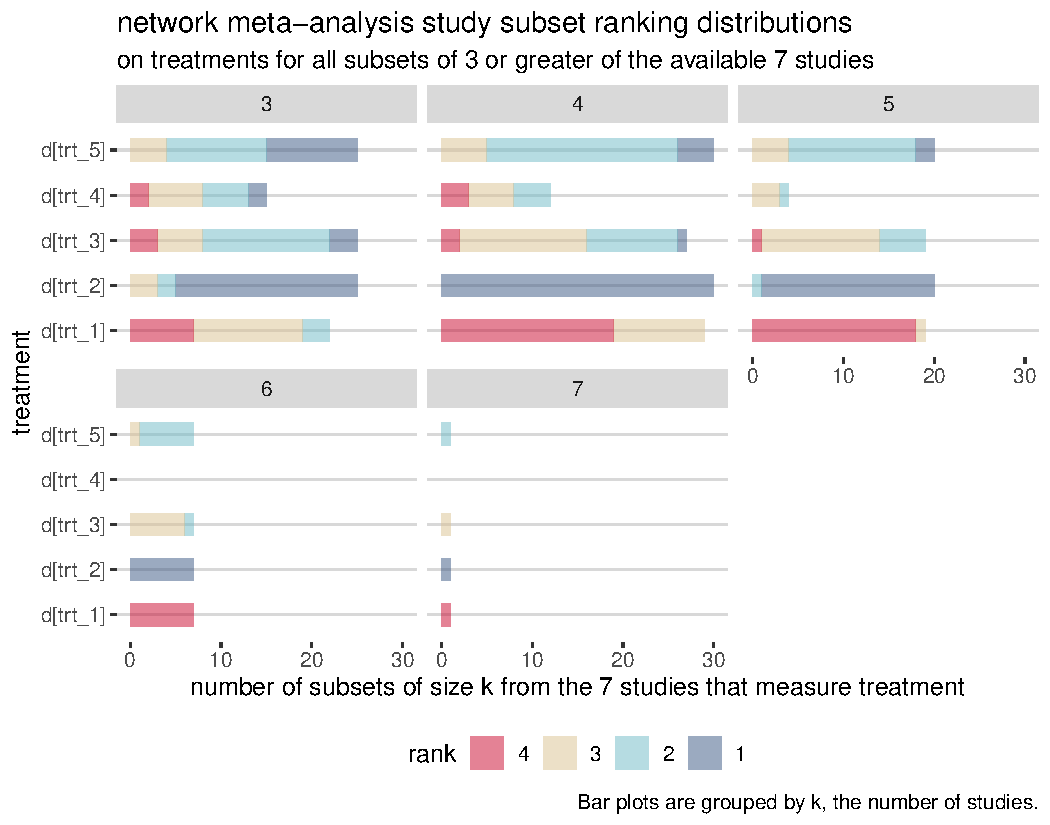
\includegraphics[width=\maxwidth]{figure/leavem-1} 

\end{knitrout}

\caption{Rankings for leave $m$ out analyses, where $m = 0, \dots, 4$ studies omitted from the total 7 studies available.}
\label{fig:leavem}
\end{figure}

Unsurprisingly, the ranking are in agreeement when including all seven studies, with treatment 2 predicted to have the greatest reduction in the measure of interest, the mean off-time reduction in patients given dopamine agonists as adjunct therapy in Parkinson's disease~\cite{phillippo_multinma_2020}. And as treatment 2 dominates in all subgroups, we surmise that there is confidence in the meta-analytic recommendation of treatment 2.

However, other possible inferences do exist in these rankings, supposing we did not have all seven studies, and it is easy to see how a different conclusion might be drawn. Furthermore, another drawback is that whilst leave $m$ studies (for $m \leqslant k$ studies) works for seven studies, this analysis is not practical for meta-analyses that aggregate a larger number of studies. Indeed, the number of network meta-analyses performed in this analysis is

\begin{knitrout}
\definecolor{shadecolor}{rgb}{0.969, 0.969, 0.969}\color{fgcolor}\begin{kframe}
\begin{verbatim}
## [1] 99
\end{verbatim}
\end{kframe}
\end{knitrout}

from seven studies. Clearly this type of analysis would become computationally intractable for larger meta-analyses.

A more robust approach would be threshold analysis, where an \textbf{invariant interval} is provided for each study, showing the interval in which the study's results will not change the ranking~\cite{phillippo_sensitivity_2018}. However, this solution is challenging, involving mathematics and \code{stan} syntax, so providing toolchains, guides, and support for practitioners will surely be helpful.

\section{Computational way station for open and inclusive scientific method development}\label{sec:comp}

% discuss contributing

% rethinking has 1243 citations

Stakeholders engage with meta-analyses in multiple ways. A lead researcher may not be interested in interacting with code repositories, but may well have thoughts about how to improve reporting for inference. A computational collaborator may wish to contribute tools for related analyses, even if not directly involved in the project.

In this section, we consider developing a toolchain for reporting a Cochrane network meta-analysis, considering how different researchers may wish to provide feedback on the implemented protocol. With increasing levels of computational complexity, we step through how researchers in various roles might contribute.

\subsection{Domain-specific principal investigator}

Consider a study where the principal investigator (PI) is a psychologist who delegates statistical analysis to other members of the team: a lead statistician, and a postdoctoral scholar under their supervision. The PI will interpret the meta-analytic findings, but will not wish to interact with code repositories. In this case, an email address of the primary maintainer (the postdoctoral scholar) of the living resource is provided for comments that can then be converted to issues by the maintainer on the repository for discussion amongst the community.

\subsection{Lead statistician}

The lead statistician will be comfortable with code, but will be time poor in comparison to the maintainer of the living resource, the postdoctoral scholar under their supervision. Whilst they may not have time to contribute they will likely have comments for the maintainer. They will likely have a GitHub account, and thus can contribute to the discussion via issues, where not only the maintainer, but any interested party can consider and add to the suggestions.

\subsection{Computational collaborators}

Now consider a computational ecologist, interested in developing tools and protocols for their own network meta-analyses. In this case, they may wish to contribute new vignettes to the website, with new toolchains, as well as develop new tools to fill the toolchain gaps.

The R package \package{usethis} includes a workflow for contributing to someone else's package\footnote{Workflow documentation available here: https://usethis.r-lib.org/articles/articles/pr-functions.html}~\cite{wickham_usethis:_2019}.

In Figure \ref{fig:workflow} is a sketch of the workflow for contributing to \package{nmareporting}, the underlying code base of the site and development. Let us suppose the ecologist is contributing an ecology-specific vignette for network meta-analysis.

\begin{figure}

\begin{knitrout}
\definecolor{shadecolor}{rgb}{0.969, 0.969, 0.969}\color{fgcolor}\begin{kframe}
\begin{alltt}
\hlkwd{library}\hlstd{(usethis)}
\hlcom{# create a fork and clone}
\hlkwd{create_from_github}\hlstd{(}\hlstr{"softloud/nmareporting"}\hlstd{)}
\hlcom{# create a branch for the specific contribution}
\hlkwd{pr_init}\hlstd{(}\hlstr{"ecovignette"}\hlstd{)}
\hlcom{#}
\hlcom{# ecologist then writes vignette}
\hlcom{#}
\hlcom{# contribute the vignette to the code repository}
\hlkwd{pr_push}\hlstd{()}
\hlcom{#}
\hlcom{# waits for maintainer to merge}
\hlcom{#}
\hlcom{# once the maintainer has merged}
\hlkwd{pr_finish}\hlstd{()}
\end{alltt}
\end{kframe}
\end{knitrout}

\caption{A workflow for contributing to the \package{nmareporting} computational way station.}
\label{fig:workflow}
\end{figure}

\section{Conclusion}

In the era of big data and rapid-fire advances in statistical software, research is still adapting to what, in fact, constitutes a useful research artifact. Mathematical algorithms are conventionally implemented via software. Computational way stations provide a meeting point, between a scholar's inception of an analysis technique, and it's formalisation in scientific protocol.


%%% bibliography
\bibliographystyle{plain}
\bibliography{references}

\end{document}
